%----------------------------------------
% Preamble to set up the document
%----------------------------------------
\documentclass{article}

% set up packages (you shouldn't need to touch this)
\usepackage{graphicx}  % required to insert images
\usepackage{hyperref}  % for hyperlinks
\usepackage[svgnames]{xcolor}  % to change hyperlink colors
\colorlet{linkcolour}{DarkBlue}
\hypersetup{colorlinks=true, linkcolor=linkcolour, citecolor=linkcolour, urlcolor=linkcolour,}

% Margins
\topmargin=-0.45in
\evensidemargin=0in
\oddsidemargin=0in
\textwidth=6.5in
\textheight=9.0in
\headsep=0.25in

% use a sans serif font
\renewcommand{\familydefault}{\sfdefault}

%----------------------------------------
% Step 1: Edit the lecture title
%----------------------------------------
\title{
Lecture 2: Counting \\  % Lecture title
Modeling Social Data, Spring 2017 \\   % Course title
Columbia University                    % School
}

%----------------------------------------
% Step 2: Edit your name and the date
%----------------------------------------
\author{bh2589}                     % Scribe's name
\date{January 27, 2017}                % Lecture date

\begin{document}

\maketitle


%----------------------------------------
% Step 3:
% Rename uni.tex to match your uni,
% edit the filename accordingly below,
% and put your notes in this file
%----------------------------------------
%----------------------------------------
% Write your notes here
%----------------------------------------

\section{Why counting?}

~~~~We can get some inspirations from the following example.

\textbf{E.g.} 2016 American Presidential Polls

Suppose we want to investigate the relationship between the election result and some related factors, such as: Age, Sex, Race, Party and etc. (i.e. P(Support|Age, Sex, Race, Party…)), and we categorize Age into 100 groups(1-99, 100+ ), Sex into 2 groups(Male/Female) , Race into 5 groups(White/Black/Asian/Hispanic/Others), Party into 3 groups(Republican/ Democratic/Independent), so there should be 100*2*5*3 = 3000 groups in total theoretically. However, normally by doing surveys, we can only collect around 1000 responses of which the number is much less than the number of groups we want to investigate.
~\\

\textbf{So here is the problem:}It is difficult to obtain reliable estimates due to small sample sizes or sparsity.

By means of counting, we can solve this problem.
~\\

\textbf{Potential solutions:}
\begin{enumerate}
\item Sacrifice granularity for precision, by binning observations into larger, but fewer groups, so that the total number of groups can be significantly decreased.

\textbf{E.g.} Bin Age from 100 groups(1-100 years old) in to fewer groups(like 5 groups: 18-29, 30-49, 50-64, 65+), then the total number of groups can be decreased by 20 times.

\item Develop more sophisticated methods that generalize well form small samples.

\textbf{E.g.} Fit a model like:  Support = $\beta_0$ + $\beta_1Age$ + $\beta_2Age^2$ + $...$

~~~~~~`Rather than:  Support= $\beta_0$ + $\beta_1Age$ + $...$

\item Obtain larger samples through other means, so we can just count and divide to make estimates via relative frequencies.

\textbf{E.g. }If we can collect around 1 million responses, we can have more than 100 responses for each group, so that we can make a good estimate of support within a few percentage points.
\end{enumerate}


\begin{itemize}
\item \textbf{Advantages and Disadvantages}
\end{itemize}
\begin{enumerate}
\item The good:

Shift away from sophisticated statistical methods on small samples to simpler methods on large samples.

\item The bad:

Even simple methods are computationally challenging at large scales.
\end{enumerate}

\section{ How to count? (Counting at small/medium scales on a single machine.) }


\begin{itemize}
\item \textbf{Procedures}
\end{itemize}

\begin{enumerate}
\item Split: Arrange observations into groups of interest.
\item Apply: Compute distributions and statistics within each group.
\item Combine: Collect results across groups.
\end{enumerate}

\textbf{E.g. }Calculating the means of the numbers in various groups (Assume there are N numbers in total, and they are from three different groups A, B, C)

\begin{figure}[ht]
  \begin{center}
    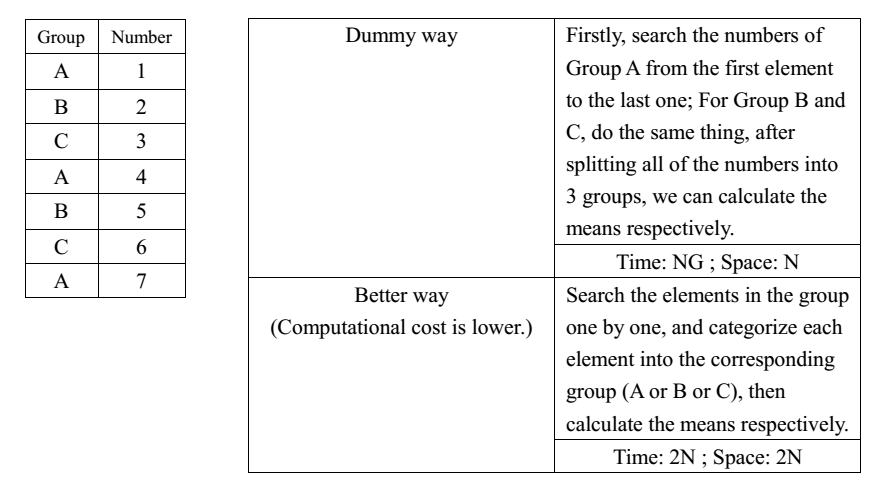
\includegraphics[width=0.6\textwidth]{figures/scribe_notes.png}
    \label{fig:scribe_notes}
  \end{center}
\end{figure}

\textbf{E.g.} The generic group-by operation
Split: Mark each observation as (group, value) and place value in bucket in corresponding group.
Apply: Apply a function over values in bucket output group and result.
Combine: Combine the final results.

\textbf{E.g.} Movielens (What we only care about is how many ratings there are, not rating itself.)

\begin{figure}[ht]
  \begin{center}
    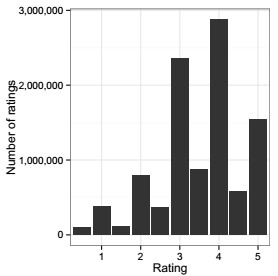
\includegraphics[width=0.4\textwidth]{figures/scribe_notes_1.png}
    \label{fig:scribe_notes_1}
  \end{center}
\end{figure}
This picture shows how many ratings there are at each star level (5 star levels in total).

The data is grouped by rating value for each group (2 groups in total in this picture).

\newpage
\begin{figure}[ht]
  \begin{center}
    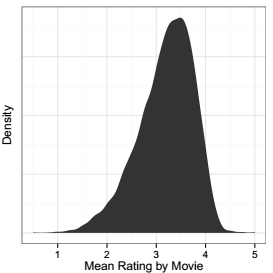
\includegraphics[width=0.4\textwidth]{figures/scribe_notes_2.png}
    \label{fig:scribe_notes_2}
  \end{center}
\end{figure}

This picture shows the distribution of the density of movies with different mean ratings.

The data is grouped by movie id for each for each group and then compute the average ratings.

\begin{figure}[ht]
  \begin{center}
    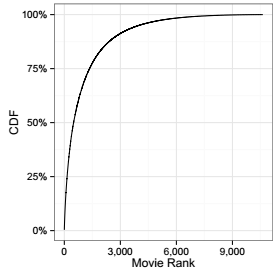
\includegraphics[width=0.4\textwidth]{figures/scribe_notes_3.png}
    \label{fig:scribe_notes_3}
  \end{center}
\end{figure}
This picture shows the fraction of ratings given to the most popular movies (with the most ratings).

The data first is grouped by movie id and then count ratings and sort by the number of ratings, finally calculate the percentage of the group size of each movie and cumulate them gradually.
\newpage
\begin{figure}[ht]
  \begin{center}
    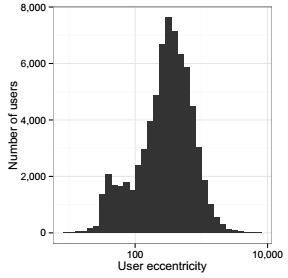
\includegraphics[width=0.4\textwidth]{figures/scribe_notes_4.png}
    \label{fig:scribe_notes_4}
  \end{center}
\end{figure}
We can infer the median rank of each user’s rated movies from the distribution from this picture.

First, we need to join movie ranks to ratings and then we group date by user id for each group, finally we compute the median movie rank.
~\\


\begin{itemize}
\item \textbf{What do we do when the full dataset exceeds available memory?}
\end{itemize}

(Wrong) Sampling: Unreliable estimates for rare groups

(Wrong) Random access from disk: It is much slower though the storage are more.

(Right) \textbf{Streaming:} Read data one observation at a time, storing only needed state.

\textbf{E.g.} The combination group-by operation

Mark each observation as (group, value), if a new group appears, we initialize the result, or we update the result for corresponding group as function of existing result and current value. Finally, for each group, we output the result.

\begin{itemize}
\item \textbf{The group-by operation}
\end{itemize}
\begin{figure}[ht]
  \begin{center}
    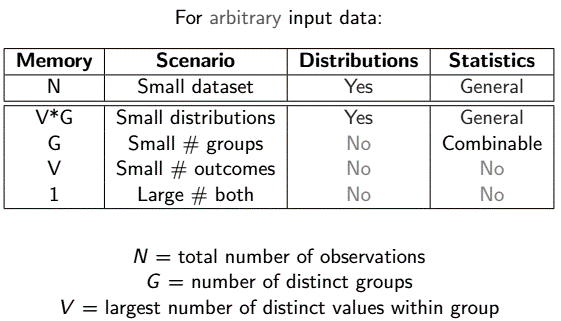
\includegraphics[width=0.4\textwidth]{figures/scribe_notes_5.png}
    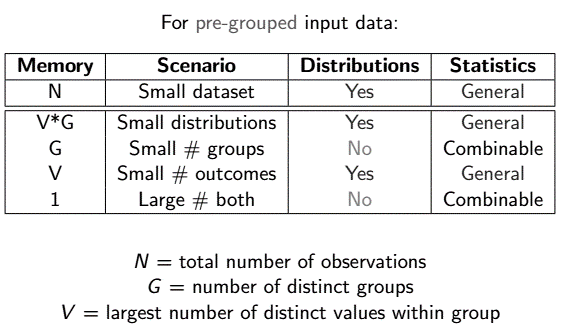
\includegraphics[width=0.4\textwidth]{figures/scribe_notes_6.png}
    \label{fig:scribe_notes_5_6}
  \end{center}
\end{figure}

\textbf{E.g. }

\textbf{Median rating by movie for Netflix:} N - 100M ratings; G - 20K movies; V - 10 half-star values.

Since V*G = 200K, we can store per-group histograms for arbitrary statistics.

\textbf{Median rating by video for YouTube:} N - 10B ratings; G - 1B videos; V - 10 half-star values.

Under this circumstance, V*G = 10B, we can’t store the data anymore because per-group histograms are too large to store in memory.

\textbf{Mean rating by video for YouTube:} N - 10B ratings; G - 1B videos; V - 10 half-star values.

In this situation, G - 1B, we can use streaming to compute combinable statistics.
                                                                              



\end{document}

%%% Local Variables:
%%% mode: latex
%%% TeX-master: t
%%% End:
